% !TEX root = ../report.tex
\chapter{Realisierung}
\begin{Spacing}{\mylinespace}

In diesem Kapitel wird die Realisierung des Projekts erläutert. Begonnen mit dem Hardwareaufbau über die Wahl der Frameworks, das Grundgerüst der Anwendung, die Integration der \textit{Kinect}-Kamera, dem Aufbau des Kamera-Systems und der Terrain-Darstellung bis zum Partikelsystem samt Physik.  \\

% !TEX root = ../report.tex
\section{Hardwareaufbau}
\begin{Spacing}{\mylinespace}

Die Hardware \\
Die Konstruktion\\
Der Aufbau

\end{Spacing}
\newpage
\clearpage
%% End Of Doc
\clearpage
% !TEX root = ../report.tex
\section{XNA Game Studio 4.0 + Kinect SDK}
\begin{Spacing}{\mylinespace}

\begin{figure}[h!]
	\centering
	
\includegraphics[width=300px]{graphics/xna.png}
\end{figure}

Für die Interaktion mit der \textit{Kinect}-Kamera und der Darstellung der Landschaft und des Partikelsystems haben wir uns für das \textit{XNA Game Studio 4.0} und das Kinect SDK von \textit{Microsoft} entschieden. Das \textit{XNA Game Studio} ist eine Programmierumgebung die auf \textit{Visual Studio} basiert und zur Entwicklung von Spielen für \textit{Windows-Phone}, \textit{XBox 360} und \textit{Windows}-basierten Computern entworfen wurde. Bestandteil des \textit{XNA Game Studio} ist das \textit{XNA Framework}, welches mehrere auf dem \textit{.Net-Framwork} basierende Bibliotheken vereint und eine sehr einfache und angenehme Schnittstelle zu diesen bereitstellt.
\\\\
Dazu gehören:

\begin{description}
	\item[DirectX] \hfill \\
	DirectX ist eine API für hochperformante Multimedia-Anwendungen und kommt meist bei der Hardware-beschleunigten Darstellung von 2D- und 3D-Grafiken zum Einsatz. 
	\item[XInput] \hfill \\
	XInput ist eine API zur Verarbeitung von Benutzereingaben über Maus, Tastatur und den \textit{XBox 360} Kontroller.
	\item[XACT] \hfill \\
	XACT(Microsoft Cross-Platform Audio Creation Tool) stellt einfache Schnittstellen zur Audiowiedergabe und der Verknüpfung von Sounds an bestimmte Ereignissen bereit.
\end{description}

In unserer Implementierung wird ausschließlich DirectX für die Darstellung und XInput für die Verarbeitung der Benutzereingaben genutzt. Zudem kommt zusätzlich das \textit{Kinect SDK} zur Ansteuerung der \textit{Kinect}-Kamera zum Einsatz, welches auch auf dem \textit{.Net-Framework} basiert und sich dadurch nahtlos und ohne weitere Anpassungen in das System integrieren lässt.

\end{Spacing}
\newpage
\clearpage
%% End Of Doc
\clearpage
% !TEX root = ../report.tex
\section{Der Renderer}
\begin{Spacing}{\mylinespace}

wie wird es erzeugt \\
einfärbung\\
höhenlinien\\


\end{Spacing}
\newpage
\clearpage
%% End Of Doc
\clearpage
% !TEX root = ../report.tex
\chapter{Kinect Integration}
\begin{Spacing}{\mylinespace}

hier wird die dll erklärt und wie sie eingebunden wird\\
kinect baut metrik vom bild um veraenderungen wahrzunehmen\\
sendet event nur wenn neues Tiefenbild vorhanden\\
tiefenbild blur\\

\end{Spacing}
\newpage
\clearpage
%% End Of Doc
\clearpage
% !TEX root = ../report.tex
\section{Terrain}
\begin{Spacing}{\mylinespace}

Nachdem wir die Kinect eingebunden hatten, das Grundgerüst des Renderers stand und wir mit Hilfe unseres Kamerasystem in der 3D Szene navigieren konnten, ging es daran uns um die Umsetzung der Terraindarstellung zu kümmern.

\subsection{Die Grundgeometrie}
Als Grundgeometrie für die Darstellung unseres Terrains erzeugen wir ein flaches reguläres Gitter, dass in der X-Z-Ebene aufgespannt ist (s. Abbildung \ref{fig:grid}). Die Größe und die Anzahl der Unterteilungen des Gitters wurde variabel gestaltet, um im späteren Verlauf der Entwicklung, einfacher unterschiedliche Konfiguration zu testen. 

\begin{figure}[h!]
	\centering
	\vspace*{10px}
	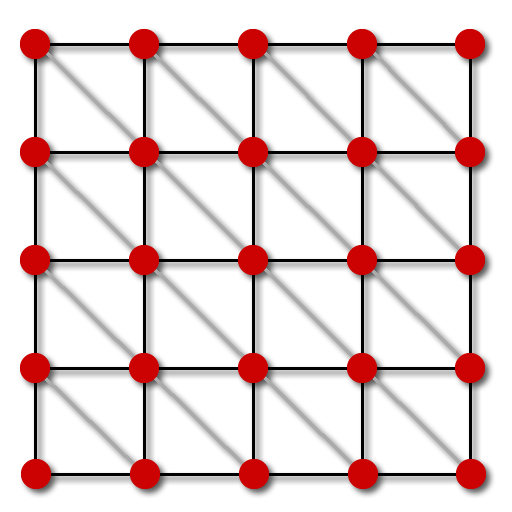
\includegraphics[width=220px]{graphics/grid.png}
	\caption{Reguläres Gitter des Terrains.}
	\label{fig:grid}
\end{figure}

\subsection{Die Höhendaten}
Um mit dem zuvor erstellten regulären Gitter ein vollständiges Abbild unserer Sandkastenlandschaft zu repräsentieren, musste nun noch ein Weg gefunden werden die von der Kinect gelieferten Höhendaten in das Model zu integrieren.
\\\\
Der erste Schritt auf diesem Weg besteht aus einer Vorverarbeitung der gelieferten Daten. Die Kinect liefert uns ein Short-Array mit 307200 Werten, was einer Auflösung von 640 x 480 Pixeln entspricht. Da der Aufbau unseres Sandkastens sowie unseres regulären Gitters allerdings quadratisch ist, müssen wir die gelieferten Daten auch auf dieses Maß beschneiden. Dazu durchlaufen wir das gelieferte Array und extrahieren daraus einen inneren quadratischen Bereich, für den, genau wie bei unserem regulären Gitter, eine variable Größe gewählt werden kann. Abbildung \ref{fig:resize} zeigt diesen Vorgang.     
\\
\begin{figure}[h!]
	\centering
	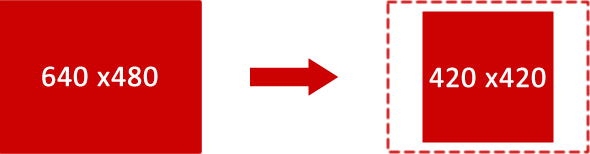
\includegraphics[width=250px]{graphics/resize.png}
	\caption{Zuschnitt der gelieferten Daten.}
	\label{fig:resize}
\end{figure}  

Um die vorarbeitenden Daten nun auf das reguläre Gitter zu übertragen, kamen zwei unterschiedliche Ansätze in Frage:
\begin{description}
	\item[1. Mit Hilfe der CPU] \hfill \\
	Beim ersten Ansatz werden die Daten direkt auf der CPU verarbeitet und in das reguläre Gitter integriert. Ein großer Nachteil dieses Ansatzes ist allerdings, dass bei jeder Aktualisierung der sogenannte \textit{VertexBuffer}, mit dessen Hilfe die Geometriedaten an die GPU übertragen werden, komplett neu aufgebaut werden muss. Dieser Vorgang ist sehr kostenintensiv und würde die Echtzeitfähigkeit unserer Anwendung stark einschränken.
	\item[2. Mit Hilfe der GPU] \hfill \\
	Beim zweiten Ansatz kann dieser kostenintensive Neuaufbau des Vertexbuffers durch moderne Shader-basierte Verfahren umgangen werden. Dazu wird aus den Daten eine Textur (Heightmap s. Abbildung \ref{fig:heightmap}) erzeugt und anschließend mit den Geometriedaten des regulären Gitters zusammen an die GPU übertragen. Im Vertex-Shader kann jetzt mit Hilfe des \textit{Vertex Texture Fetch} (VTF) Verfahrens direkt auf diese Textur und die enthaltenen Höhendaten zugegriffen und für die Manipulation der Y-Position der einzelnen Vertizes genutzt werden.
\end{description}

Entschieden haben wir uns letztendlich für den zweiten Ansatz, da er das weitaus höhere Potenzial zur Echtzeitfähigkeit bietet, welche für unsere Anwendung eine sehr wichtige Rolle spielt und darüber hinaus auch ressourcensparender ist. 

\begin{figure}[h!]
	\centering
	\vspace*{20px}
	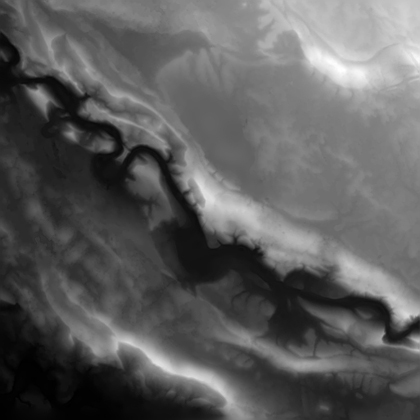
\includegraphics[width=200px]{graphics/heightmap.jpg}
	\caption{In einer Textur abgelegte Höhendaten (Heightmap).}
	\label{fig:heightmap}
\end{figure}

\subsection{Die Darstellung}
Nachdem nun die Grundgeometrie erzeugt, die Höhendaten vor verarbeitet an die GPU übertragen und die Y-Position der Vertices manipuliert wurden, können wir unser Terrain endlich nun darstellen. Einheitlich eingefärbt, bekommen wir allerdings ein Ergebnis dass nicht wirklich an eine Landschaft erinnert (s. Abbildung \ref{fig:singleColor}). 

\begin{figure}[h!]
	\centering
	\vspace*{20px}
	
\includegraphics[width=320px]{graphics/singleColor.png}
	\caption{Darstellung mit nur einer Farbe.}
	\label{fig:singleColor}
\end{figure}

Dieses Erscheinungsbild lässt sich durch ein fehlendes Beleuchtungssystem und die dadurch fehlende Schattierung der Szene erklären. Da die Implementierung eines kompletten Beleuchtungssystems für unsere Anwendung allerdings wenig Sinn machen würde, lösen wir das oben gezeigte Darstellungsproblem mit Hilfe von verschiedenen Farben für die unterschiedlichen Höhenwerte. Die einfachste Umsetzung dafür wäre direkt die Farbwerte aus der Höhentextur zu nutzen, wodurch ein Graustufenverlauf von dunkel (niedrig) zu hell (hoch) entstehen würde (s. Abbildung \ref{fig:differentColors}a). Hierdurch erhalten wir zwar eine korrekte Darstellung unseres Terrains, jedoch sind Graustufen mehr als ungeeignet für die spätere Projektion auf den Sand. Aus diesem Grund haben wir eine Möglichkeit zur benutzerdefinierten Wahl des Farbverlaufs implementiert. Diese besteht aus vier frei wählbaren Farben für vier unterschiedliche Höhenbereiche welche im Shader linear interpoliert werden (s. Abbildung \ref{fig:differentColors}b,c).    

\begin{figure}[h!]
	\centering
	\vspace*{30px}
	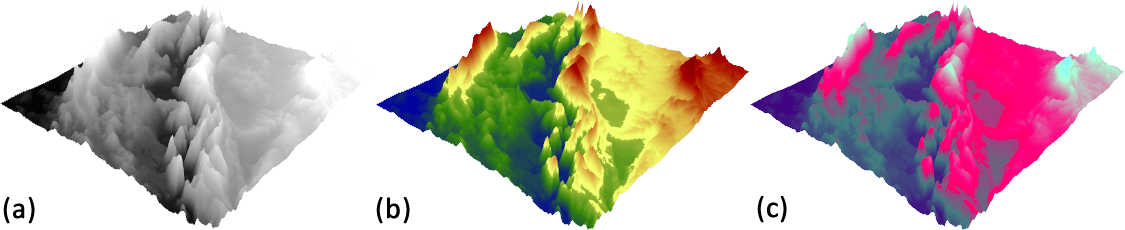
\includegraphics[width=\textwidth]{graphics/differentColors.png}
	\caption{(a) Einfärbung anhand der Höhentextur. (b, c) Einfärbung anhand eines benutzerdefinierten Farbverlaufs.}
	\label{fig:differentColors}
\end{figure}

Um die Höhenunterschiede bei der Projektion auf den Sand noch deutlicher zu machen, haben wir am Ende des Semesters noch mit der Darstellung von Höhenlinien experimentiert (s. Abbildung \ref{fig:contourLines}). Diese verbinden in bestimmten Abständen alle Punkte mit den gleichen Höhenwerten. Die aktuelle Implementierung ist noch nicht perfekt und benötigt noch einiges an Nachbearbeitung, aber schon jetzt kann man die Vorteile bei der Projektion auf den Sand erkennen. 

\begin{figure}[h!]
	\centering
	\vspace*{50px}
	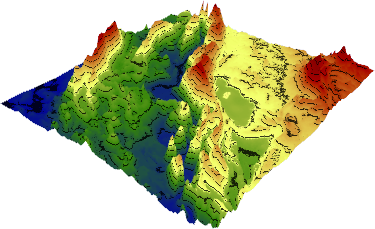
\includegraphics[width=400px]{graphics/contourLines.png}
	\caption{Experimentelle Darstellung mit zusätzlichen Höhenlinien.}
	\label{fig:contourLines}
\end{figure}


\end{Spacing}
\newpage
\clearpage
%% End Of Doc
\clearpage
% !TEX root = ../report.tex
\section{Das Kamerasystem}
\begin{Spacing}{\mylinespace}

wie wird es erzeugt \\
einfärbung\\
höhenlinien\\


\end{Spacing}
\newpage
\clearpage
%% End Of Doc
\clearpage
% !TEX root = ../report.tex
\section{Partikelsystem}
\begin{Spacing}{\mylinespace}

Es gibt verschiedene Möglichkeiten ein Partikelsystem zu realisieren.
In unserem Anwendungsfall haben wir uns dafür entschieden Visualisierung und Physik zu trennen.
Dies führt dazu, das es möglich ist, ohne große Abhängigkeiten voneinander parallel zu entwickeln.

\subsection{Die Physik (Physik-Engine)}
Damit die Partikel möglichst realitätsgetreu sich durch die Szene bewegen, benötigt der Computer die Information wie sich die entsprechenden Partikel verhalten sollen.
Dies bedeutet das physikalische Gesetze auf mathematische Funktionen abgebildet werden müssen.
Durch diese Abbildung werden die Bewegungsabläufe der Partikel gesteuert.
Um die Echtzeitfähigkeit des Systems sicher zu stellen müssen meist die Abbildungen (Gesetze) durch ein paar Tricks vereinfacht werden um Rechenkraft zu sparen.

Die Physik-Engine hat genau diese Aufgaben; Sie bewegt die Partikel durch den Raum, erkennt Kollisionen und bildet Gesetzte der \ref{Reflektion} ab.
Durch die hohe Unabhängigkeit von den einzelnen Partikeln eignet sich eine GPU besonders gut zum berechnen entsprechender Gesetze.
Wir haben uns dennoch im aktuellen Projektstatus dazu entschieden die Berechnungen auf der CPU durchzuführen.
Der Grund hierfür liegt in der Problematik das es nicht möglich ist Berechnungen welche auf der GPU stattfinden genauer zu untersuchen bzw. zu Debuggen.

\subsection{Der Renderer (Draw-Engine)}
Der Renderer ist der zweite Teil unseres Partikelsystems. Seine Aufgabe liegt darin, für jedes einzelnes Partikel die Eigenschaften (Farbe,Kraft,Größe,...) für den Benutzer zu visualisieren.
Hierbei wird lediglich lesend auf den vorhandene Datenbestand zugegriffen.
Auch hier ist eine hohe Parallelität möglich, denn jedes Partikel stellt eine unabhängige Einheit dar.
Somit ist es möglich mit Hilfe von DirektX einen Shader für die GPU zu schreiben. 
Dieser erlaubt es, das alle Shader-Units der GPU zusammen an einem Frame arbeiten. 

\end{Spacing}
\newpage
\clearpage
%% End Of Doc
\clearpage
% !TEX root = ../report.tex
\section{Die Physik}
\begin{Spacing}{\mylinespace} 

\end{Spacing}
\newpage
\clearpage
%% End Of Doc
\clearpage
% !TEX root = ../report.tex
\section{GUI}
\begin{Spacing}{\mylinespace}

anbindung der elemente \\
darstellungsart bla blub\\
integration xna in gui etc\\
kallibration der sandkiste\\


\end{Spacing}
\newpage
\clearpage
%% End Of Doc
\clearpage

\end{Spacing}
\newpage
\clearpage
%% End Of Doc